% \begin{frame}[t]{Recapitulando}
%     \pause
%     \begin{comando}
%             \texttt{git status}
%     \end{comando}

%     \vspace{.4em}

%     \begin{columns}[t]
%         \begin{column}{0.05\textwidth}

%         \end{column}
%         \begin{column}{0.90\textwidth}
%             \pause
%             \hspace{-.25em}\texttt{Changes to be commited:}

%             \pause
%             \begin{block}{La clase anterior, aprendimos cómo:}
%                 \begin{itemize}
%                     \pause
%                     \item Obtener una copia local de un repositorio (\texttt{git\alt<-5>{...}{ clone}}).
%                     \pause\pause
%                     \item Iniciar un repositorio vacío (\texttt{git\alt<-7>{...}{ init}}).
%                     \pause\pause
%                     \item Marcar cambios como preparados o \textit{staged} (\texttt{git\alt<-9>{...}{ add}}),
%                     \pause\pause y confirmar estos cambios (\texttt{git\alt<-11>{...}{ commit}}).
%                     \pause\pause
%                     \item Ver el estado actual de nuestros cambios (\texttt{git\alt<-13>{...}{ status}}).
%                     \pause\pause
%                     \item Enviar nuestros cambios a un repositorio remoto (\texttt{git\alt<-15>{...}{ push}}) \pause\pause y
%                     bajarnos los cambios a nuestro repositorio local (\texttt{git\alt<-17>{...}{ pull}}).
%                     \pause\pause
%                     \item Resolver los conflictos que pueden presentarse al trabajar de forma colaborativa.
%                 \end{itemize}
%             \end{block}

%         \end{column}
%         \begin{column}{0.05\textwidth}

%         \end{column}
%     \end{columns}

% \end{frame}

% \begin{frame}[t]{Recapitulando}
% \begin{comando}
%     \texttt{git status}
% \end{comando}
    
%     \vspace{.4em}

%     \begin{columns}[t]
%         \begin{column}{0.05\textwidth}

%         \end{column}
%         \begin{column}{0.90\textwidth}
%             \hspace{-.25em}\texttt{Untracked files:}

%             \pause
%             \begin{block}{Hoy vamos a ver:}
%                 \begin{itemize}
%                     \item Comandos para mover y eliminar archivos.
%                     \item Comandos para inspeccionar cambios anteriores.
%                     \item Ramificaciones (o \textit{branches}).
%                     \item Algunos comandos un poco más avanzados.
%                     \item \textit{Bonus track}.
%                 \end{itemize}
%             \end{block}

%         \end{column}
%         \begin{column}{0.05\textwidth}

%         \end{column}
%     \end{columns}

% \end{frame}

% ejercicio en el que tengan que hacer algo de lo que se arrepientan.
% hacen un add de 2 archivos
% x ejemplo, uno solo edita los dos archivos 
% tira un diff
% pero quiere borrarlo, moverlo, unstagearlo.
% ejercicio con restore

% editas los dos. git diff (diff los 2 archivos)
% queres restaurar uno. git restore
% git diff
% commit, push, pull

% falta acá escribir algo de motivacion de por que usamos ramas
% features distintas del mismo proyecto, probablemente en el mismo archivo
% al terminar deberan hacer un merge, pero una sola vez

% introducir conflictos
% corto, ya practicamos bastante
% ambos crean un archivo con el mismo nombre y distinto contenido.
% intentan pushear  caos

% por eso usamos branches

% ejercicios
% hay un jefe medio bobo que pushea todo en main mientras vos estabas trabajando. intentas hacer un push y no te deja, haces un pull y hay mil conflictos y no anda nada.
% solucion: trabajar en tu rama, y si tu jefe pushea, no pasa nada.
\begin{frame}[t]{Ramificaciones en Git}

    % Git es distribuido

    Una \textbf{rama} (o \textit{branch}) en Git representa una línea independiente de desarrollo.
    Al crear nuevas ramas, podemos pensar que nuestro proyecto diverge en dos distintos:
    los cambios que hagamos en uno no impactan al otro.

    \pause
    \vspace{0.5em}
    Un ejemplo visual:

    \begin{figure}[ht]
        \begin{center}
            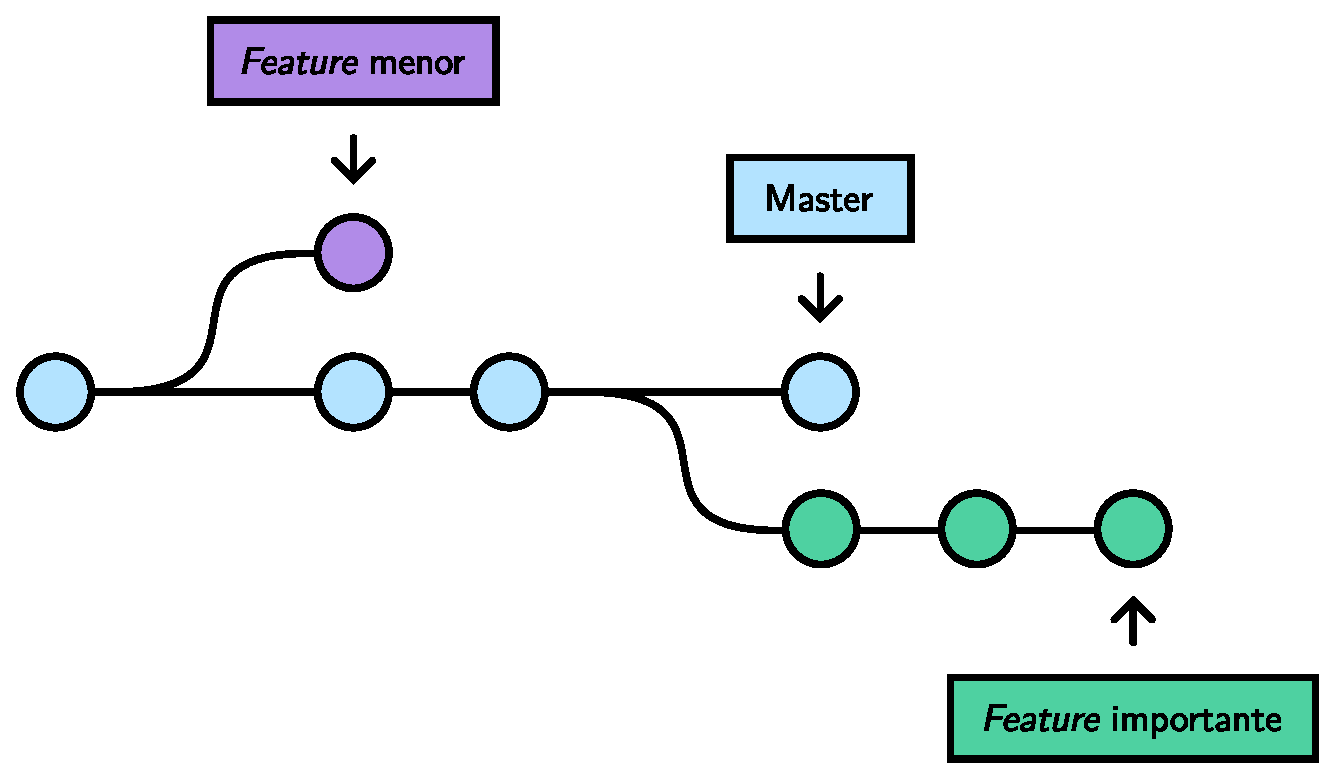
\includegraphics[height=1.5in]{images/branch.pdf}
        \end{center}
    \end{figure}

\end{frame}

% \begin{frame}{Conceptos claves}
%         \begin{itemize}
%             \item {\textit{main:} rama predeterminada que se crea automáticamente cuando se crea un repositorio.}
%             \pause
%             \item {\textit{origin:} nombre predeterminado que recibe el repositorio remoto principal contra el que trabajamos.}
%             \pause
%             \item {\textit{HEAD:} commit en el que está tu repositorio posicionado en cada momento.}
%         \end{itemize} 
% \end{frame}

\begin{frame}[t]{Creando ramas}
    \begin{comando}
        git branch
    \end{comando}

    \pause
    \begin{block}{}
        Para crear una rama nueva, podemos ejecutar \texttt{git branch [nombre de la rama]}.

        \vspace{.4em}

        Nótese que este comando no nos mueve a la nueva rama, solo la crea.

        \vspace{.4em}

        Para ver las ramas de nuestro repositorio local, podemos ejecutar \texttt{git branch}.
    \end{block}

    \pause
    \begin{ejercicio}{Ejercicio}
        Crear una rama llamada ``prueba'' en algún repo de la clase pasada.
    \end{ejercicio}

\end{frame}

% git chechout -v

\begin{frame}[t]{Cambiando de rama}
    \begin{comando}
        git checkout
    \end{comando}

    \pause
    \begin{block}{}
        Para cambiar de rama, podemos ejecutar \texttt{git checkout [nombre de la rama]}.
    \end{block}

    \pause
    \vspace{0.5em}
    Un ejemplo visual:
    \vspace{-1.6em}

    \only<3-3>{
        \begin{figure}[ht]
            \begin{center}
                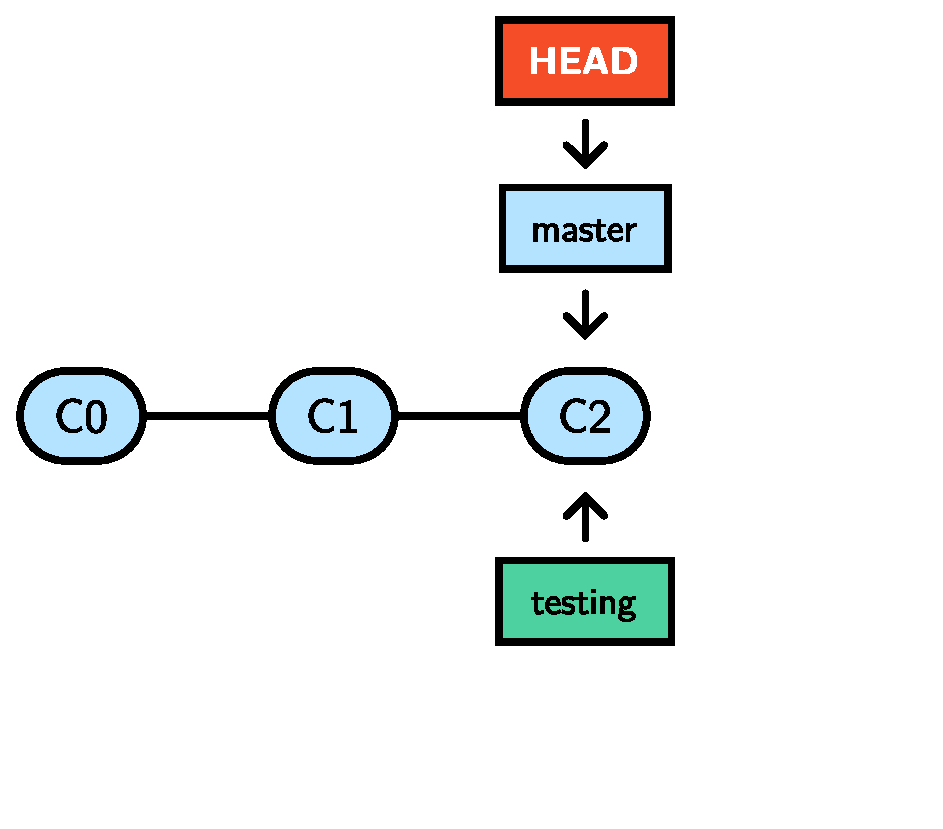
\includegraphics[height=1.6in]{images/checkout-branch-0.pdf}
            \end{center}
            \caption{}
        \end{figure}
    }

    \only<4-4>{
        \begin{figure}[ht]
            \begin{center}
                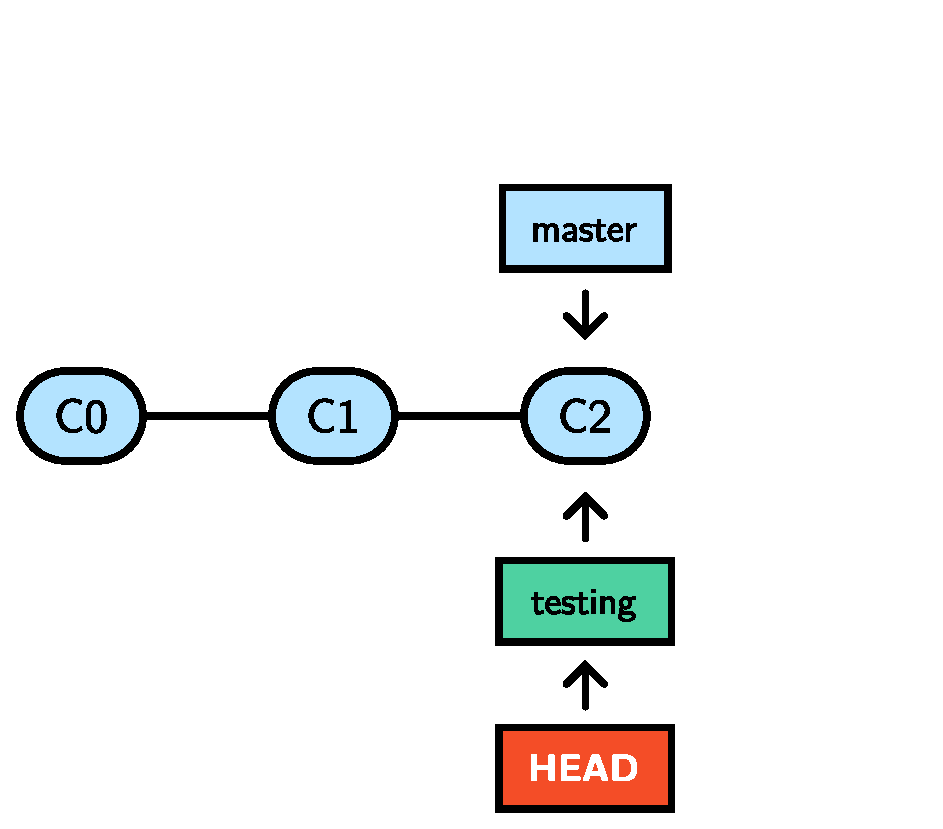
\includegraphics[height=1.6in]{images/checkout-branch-1.pdf}
            \end{center}
            \caption{Acá cambiamos a la rama ``testing'', ejecutando \texttt{git checkout testing}.}
        \end{figure}
    }

    \uncover<5-5>{
        \begin{figure}[ht]
            \begin{center}
                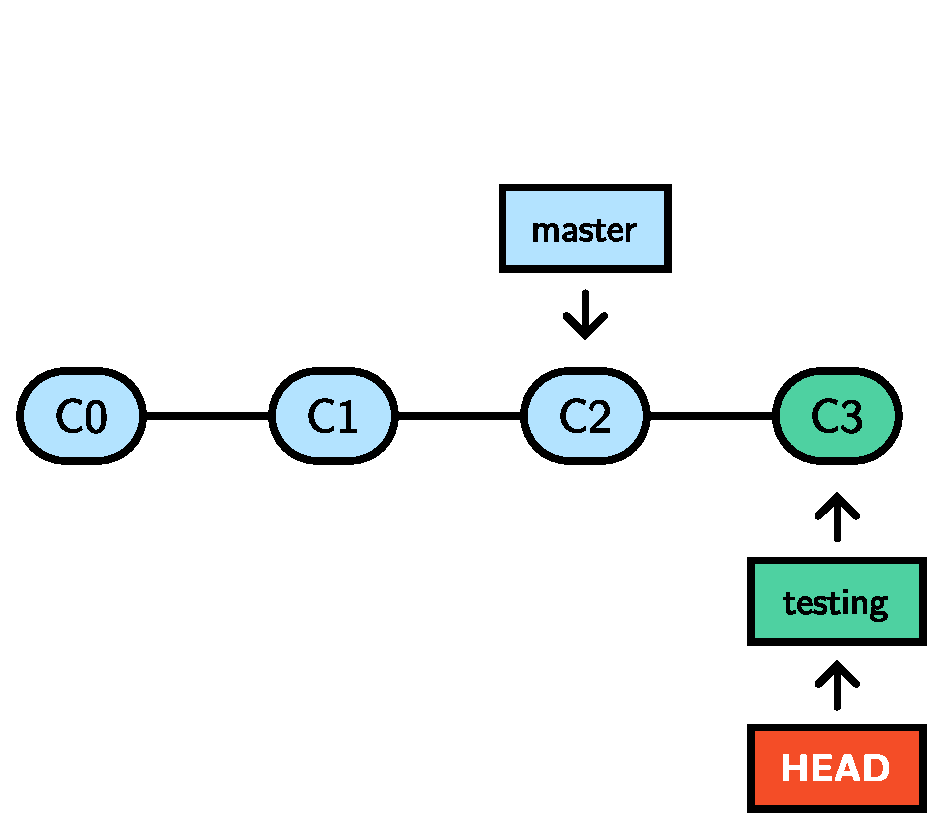
\includegraphics[height=1.6in]{images/checkout-branch-2.pdf}
            \end{center}
            \caption{Y los siguientes \textit{commits} serán agregados a la rama ``testing''.}
        \end{figure}
    }

\end{frame}

\begin{frame}[t]{Fusionando ramas}
    \begin{comando}
        git merge
    \end{comando}

    \pause
    \only<2-2>{
        \begin{block}{}
            Nos permite fusionar las historias de dos ramas distintas (podría haber conflictos).

            \vspace{.4em}

            La sintaxis es: \texttt{git merge [nombre de la rama a fusionar]}.

            \vspace{.4em}

            \textbf{Importante:} este comando fusiona la rama que le decimos
            \textbf{en la rama en la que estamos parados}.
        \end{block}
    }

    \pause
    Un ejemplo visual:
    \only<3-3> {
        \begin{figure}[ht]
            \begin{center}
                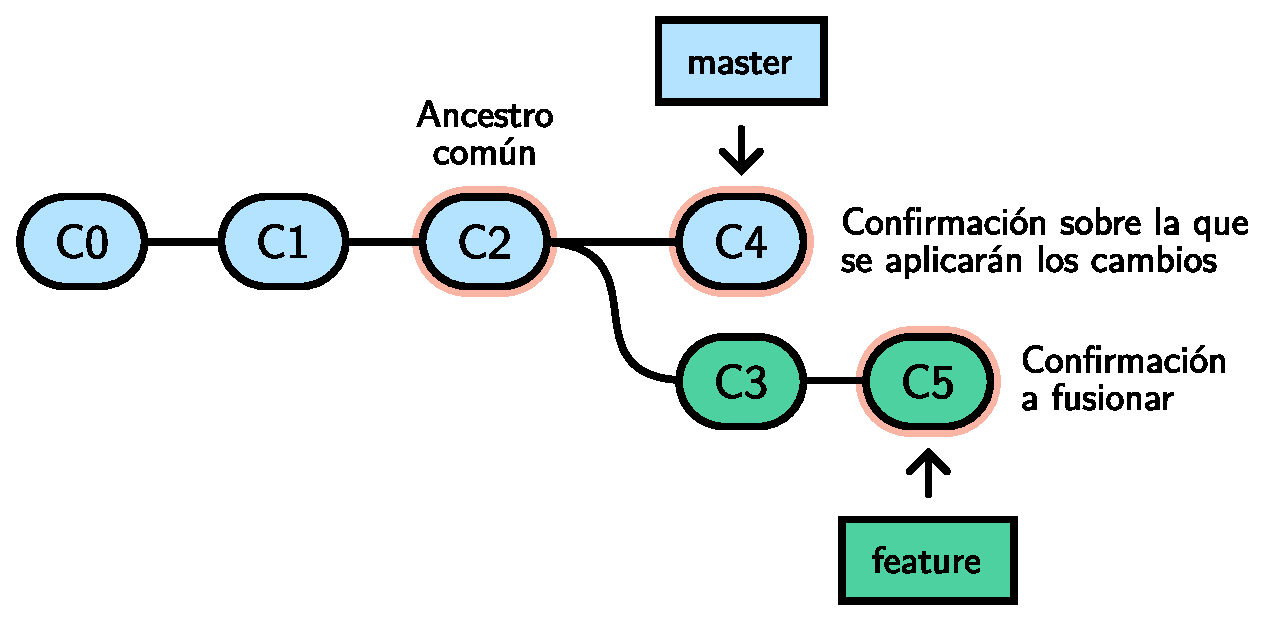
\includegraphics[height=1.5in]{images/merge-branch-0.pdf}
            \end{center}
            \caption{Antes del \textit{merge}.}
        \end{figure}
    }
    \only<4-4> {
        \begin{figure}[ht]
            \begin{center}
                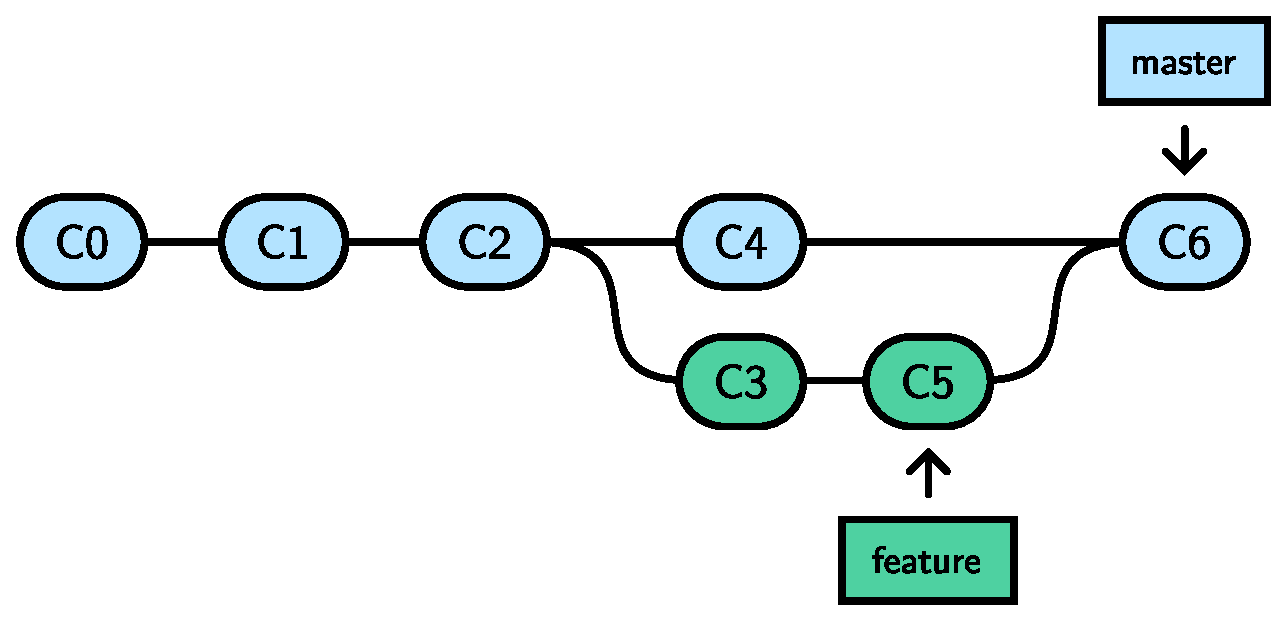
\includegraphics[height=1.5in]{images/merge-branch-1.pdf}
            \end{center}
            \caption{Después de pararnos en la rama ``master'' (\texttt{git checkout master}) y haber fusionado la rama ``feature'' (\texttt{git merge feature}).}
        \end{figure}
    }
\end{frame}

\begin{frame}[t]{¡A practicar!}

    \pause
    \begin{block}{Pero antes de empezar...}
        Para hacer el siguiente ejercicio, vamos a trabajar con un \textbf{fork} de un repositorio.
        \pause\textit{¿Y eso?}

        \pause
        Los servidores de Git, como GitLab, nos permiten hacer \textit{fork} de proyectos. Al hacer
        esto creamos una copia de un repositorio ajeno en nuestra propia cuenta, sobre la cual
        tendremos todos los permisos para pushear libremente. Los cambios que hagamos en nuestra copia \textbf{no} impactarán
        en el repositorio original.
    \end{block}

    \pause
    \begin{center}
    \Large Ahora sí...
    \end{center}
\end{frame}

\begin{frame}[t]{¡A practicar!}
    \begin{ejercicio}{Ejercicio de a 2 máquinas (preferiblemente 2 personas): \emoji{alien} y \emoji{alien-monster}}
        \begin{enumerate}\begin{scriptsize}
            \pause
            \item \emoji{alien}: Hacer un \textit{fork} en su cuenta de \href{https://www.gitlab.com}{GitLab}
            de este repositorio: \url{https://gitlab.com/talleres-comcom/taller-git-ejercicio2}, y darle permiso a \emoji{alien-monster}
            para hacer \textit{push}.
            \pause
            \item \emoji{alien} y \emoji{alien-monster}: Obtener una copia local del repositorio de \emoji{alien}.
            \only<4>{\setcounter{enumi}{2}
            \item \emoji{alien} y \emoji{alien-monster}: El repo tiene una única rama, ``master'', donde van a encontrar un fragmento incompleto,
            de un cuento de Borges. Repartirse el trabajo: cada uno deberá completar un parrafo.

            \begin{figure}[ht]
                \begin{center}
                    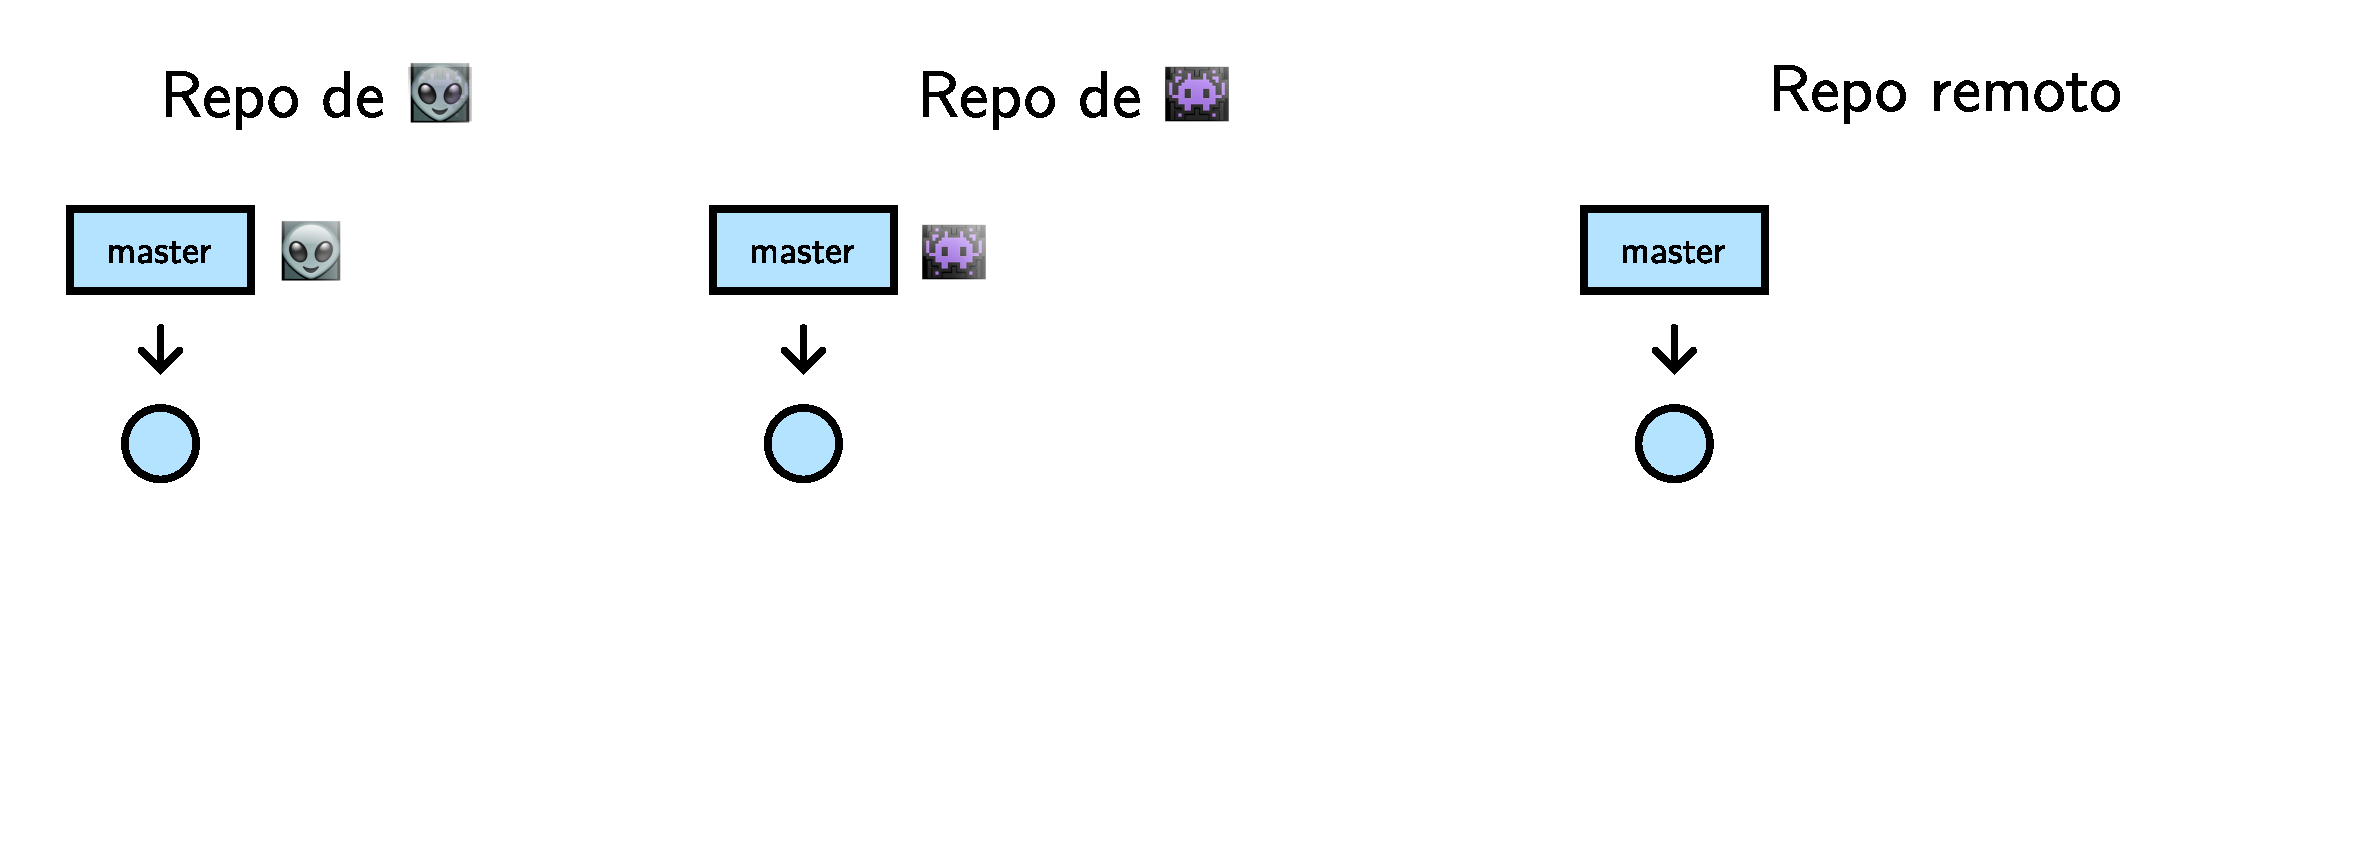
\includegraphics[height=1.7in]{images/ejercicio-clase2-1.pdf}
                \end{center}
            \end{figure}
            }
            \only<5>{\setcounter{enumi}{3}\item \emoji{alien} y \emoji{alien-monster}: Crear, cada uno, una rama propia donde harán sus modificaciones. Posicionarse
            en la rama recién creada.

            \begin{figure}[ht]
                \begin{center}
                    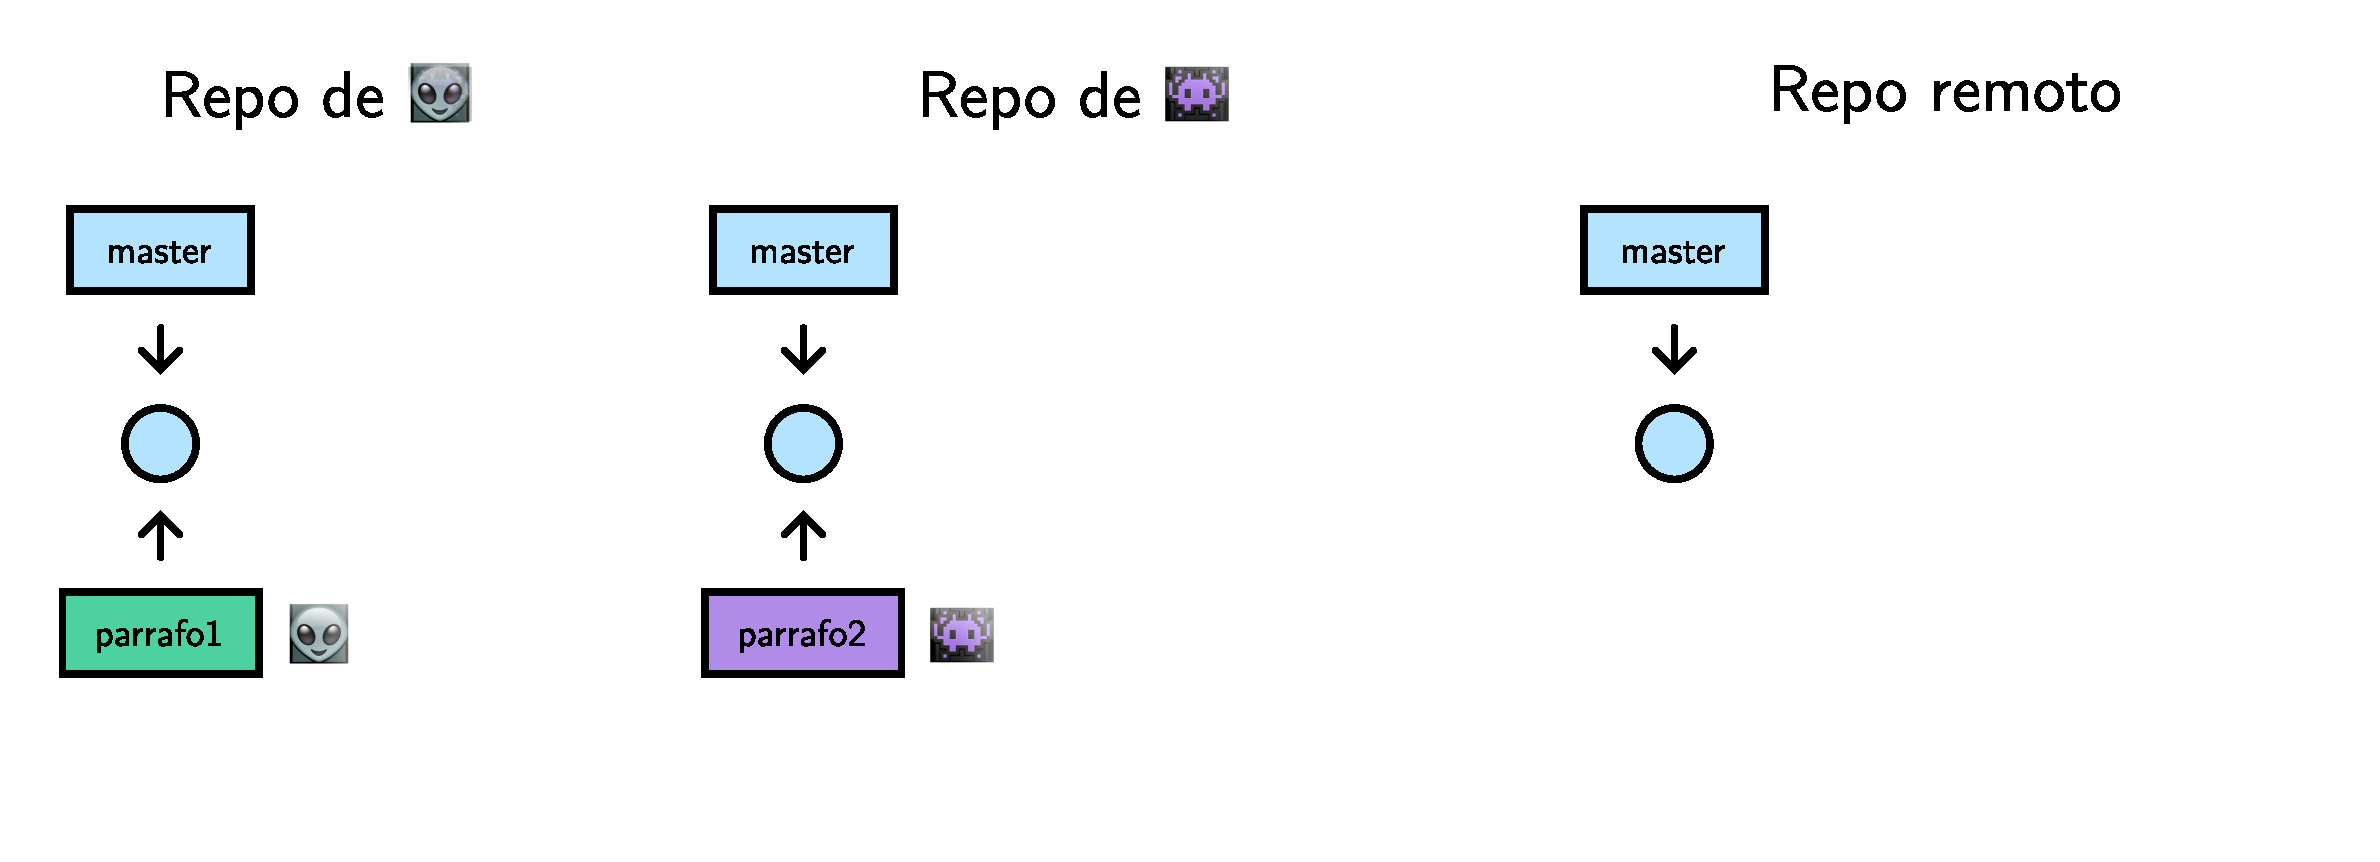
\includegraphics[height=1.7in]{images/ejercicio-clase2-2.pdf}
                \end{center}
            \end{figure}
            }
            \only<6>{\setcounter{enumi}{4}\item \emoji{alien} y \emoji{alien-monster}: Completar la parte elegida del cuento, y hacer \textit{push} de estos
            cambios en el repositorio remoto.

            \begin{figure}[ht]
                \begin{center}
                    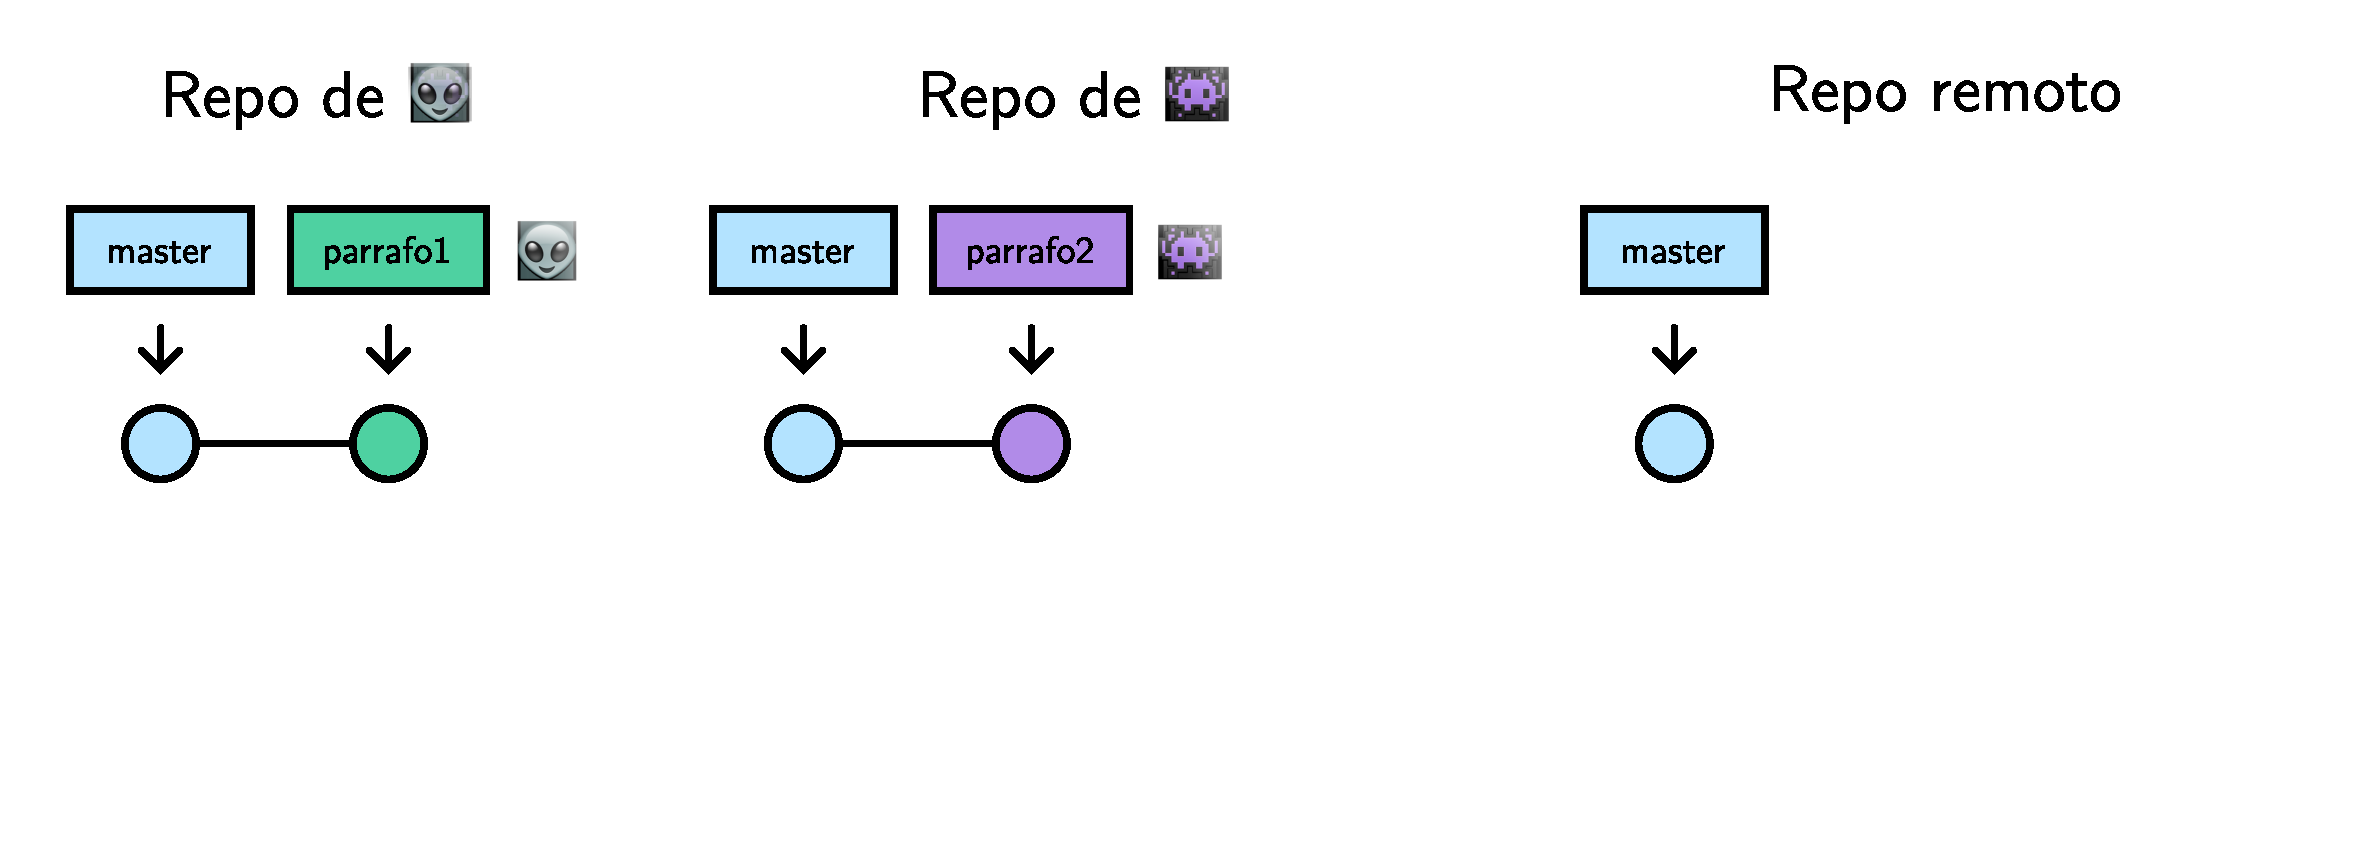
\includegraphics[height=1.7in]{images/ejercicio-clase2-3.pdf}
                \end{center}
            \end{figure}
            }
            \only<7>{\setcounter{enumi}{4}\item \emoji{alien} y \emoji{alien-monster}: Completar la parte elegida del cuento, y hacer \textit{push} de estos
            cambios en el repositorio remoto.

            \begin{figure}[ht]
                \begin{center}
                    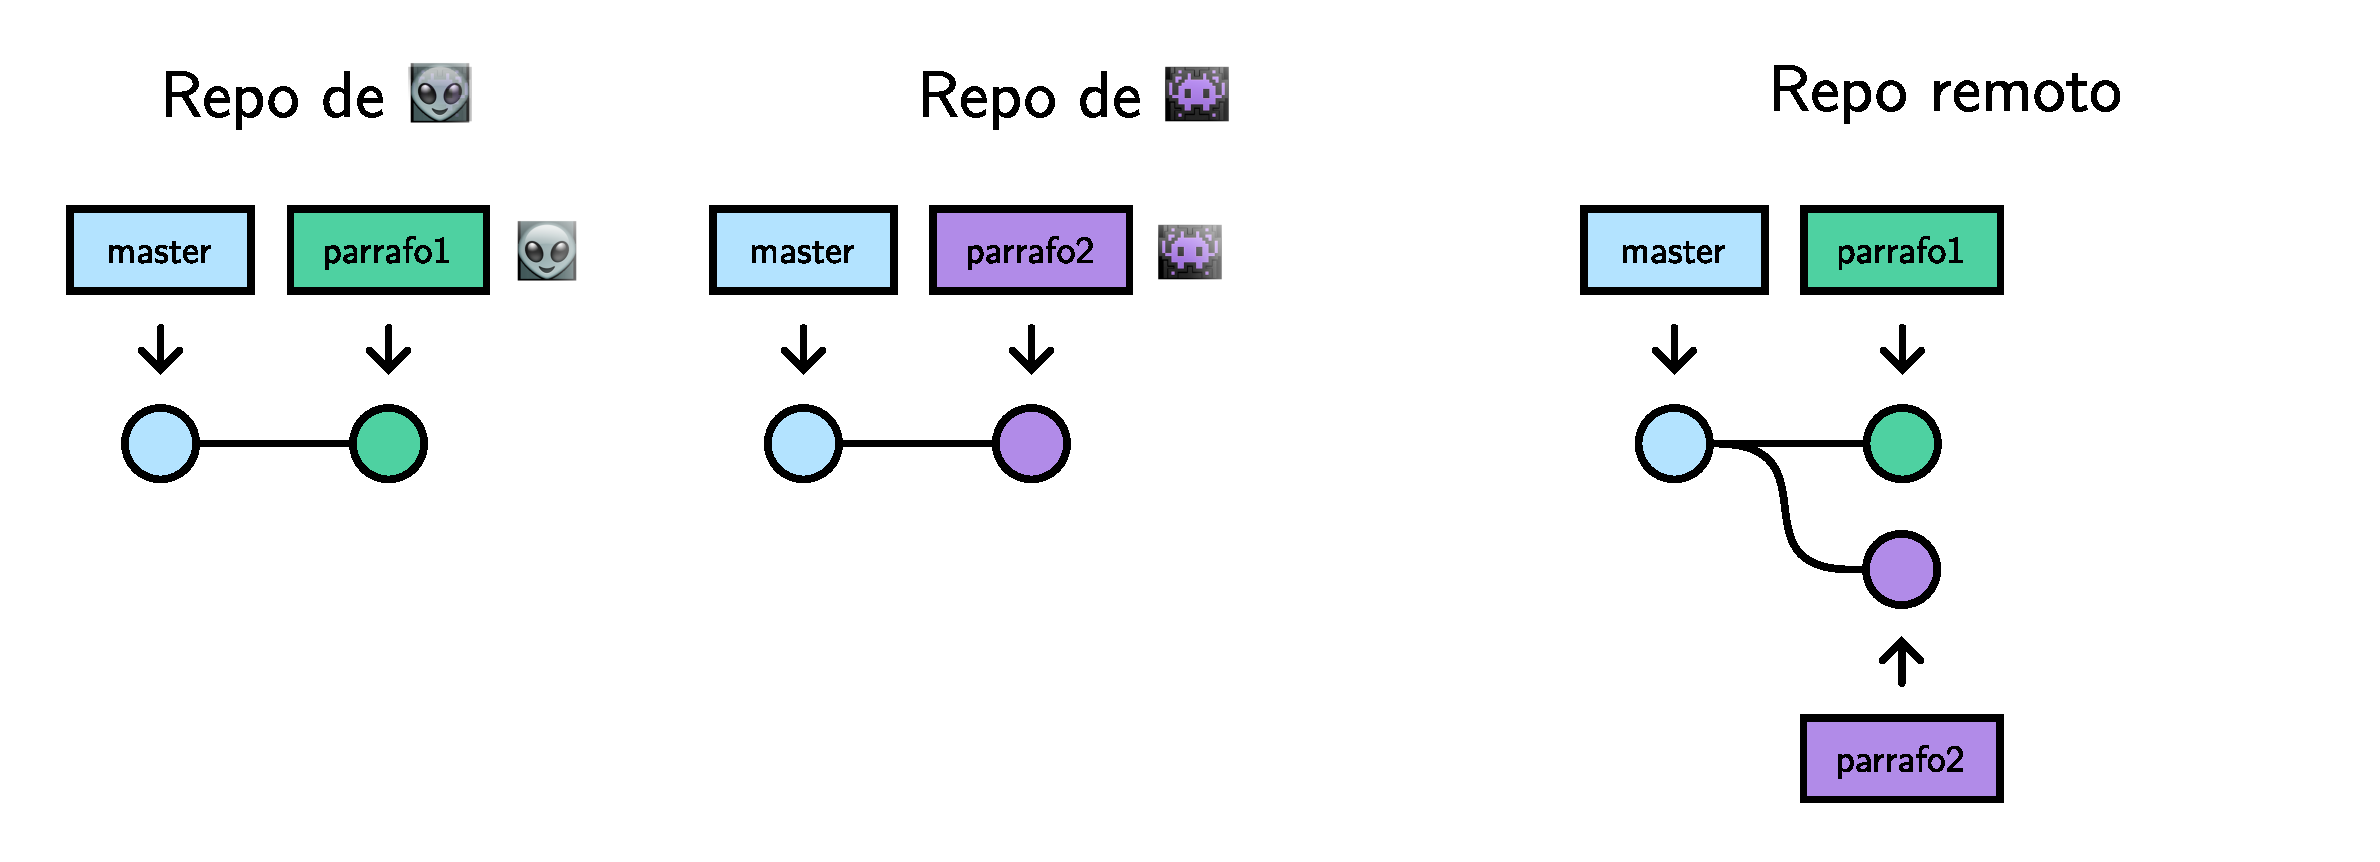
\includegraphics[height=1.7in]{images/ejercicio-clase2-4.pdf}
                \end{center}
            \end{figure}
            }
            \only<8>{\setcounter{enumi}{5}\item \emoji{alien-monster}: Traer los cambios de la rama de \emoji{alien}.

            \begin{figure}[ht]
                \begin{center}
                    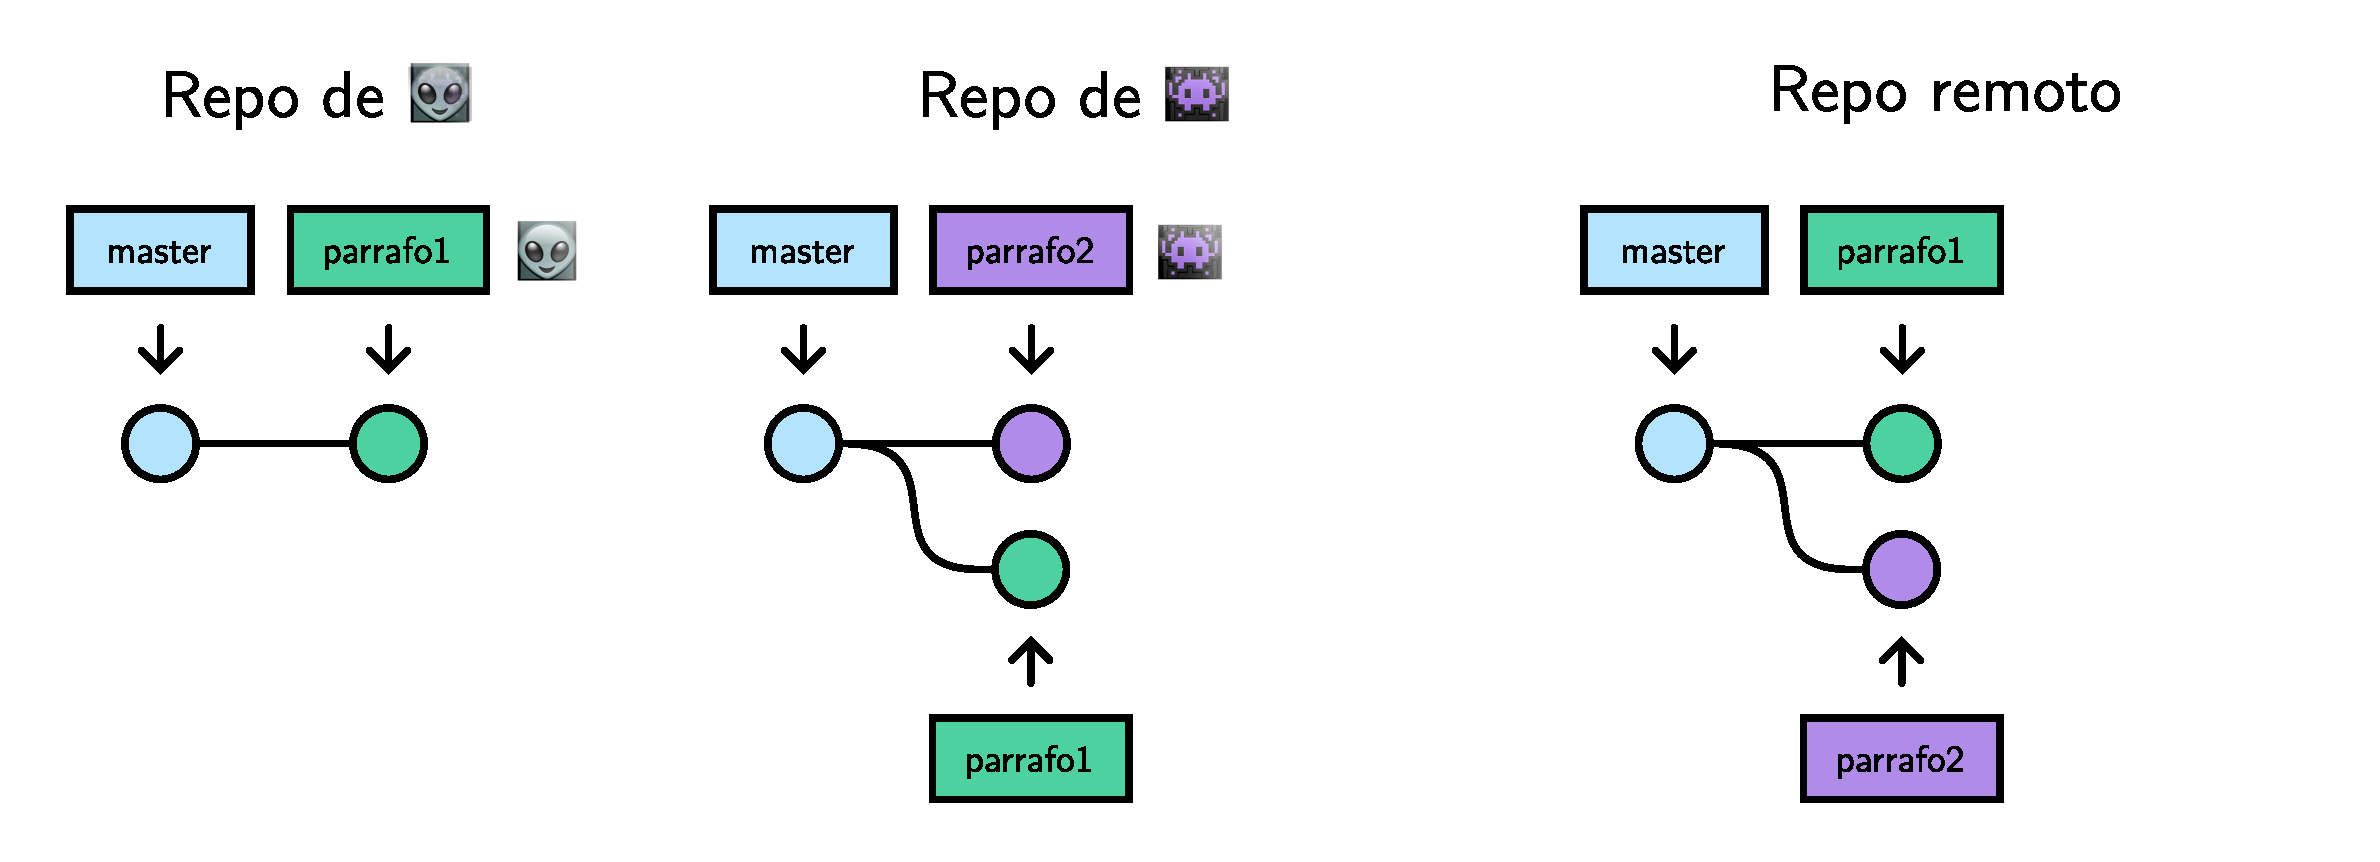
\includegraphics[height=1.7in]{images/ejercicio-clase2-7.pdf}
                \end{center}
            \end{figure}
            }
            \only<9>{\setcounter{enumi}{6}\item  \emoji{alien-monster}: Fusionar en la rama de \emoji{alien-monster} los cambios de \emoji{alien}. Enviar estos
            cambios al repositorio remoto.

            \begin{figure}[ht]
                \begin{center}
                    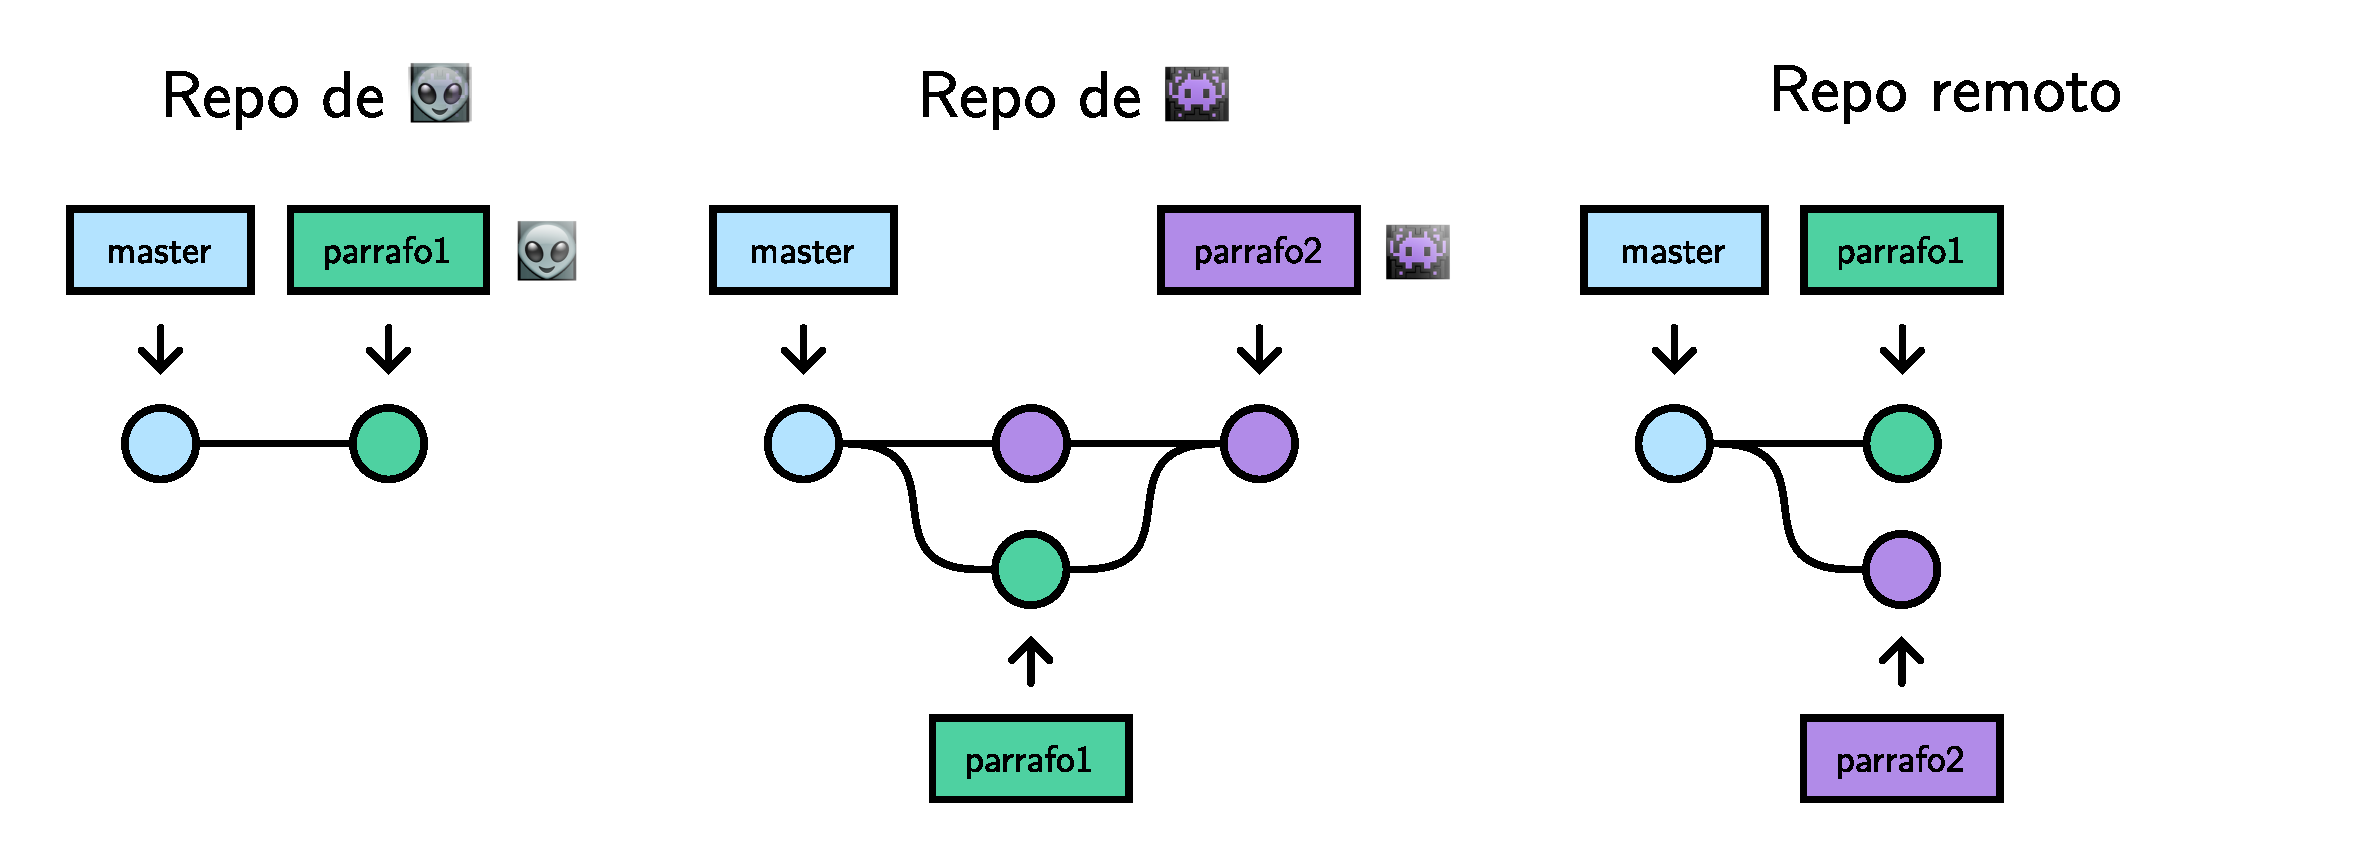
\includegraphics[height=1.7in]{images/ejercicio-clase2-8.pdf}
                \end{center}
            \end{figure}
            }
            \only<10>{\setcounter{enumi}{7}\item \emoji{alien}: Seguir los dos pasos anteriores, pero con los cambios de \emoji{alien-monster}.
            }
            \only<11>{
            \item \emoji{alien} y \emoji{alien-monster}: El repo tiene una única rama, ``master'', donde van a encontrar un fragmento incompleto,
            de un cuento de Borges. Repartirse el trabajo: cada uno deberá completar un parrafo.
            \item \emoji{alien} y \emoji{alien-monster}: Crear, cada uno, una rama propia donde harán sus modificaciones. Posicionarse
            en la rama recién creada.
            \item \emoji{alien} y \emoji{alien-monster}: Completar la parte elegida del cuento, y hacer \textit{push} de estos
            cambios en el repositorio remoto.
            \item \emoji{alien-monster}: Traer los cambios de la rama de \emoji{alien}.
            \item \emoji{alien-monster}: Fusionar en la rama de \emoji{alien-monster} los cambios de \emoji{alien}. Enviar estos
            cambios al repositorio remoto.
            \item \emoji{alien}: Seguir los dos pasos anteriores, pero con los cambios de \emoji{alien-monster}.
            }
        \end{scriptsize}\end{enumerate}
    \end{ejercicio}

\end{frame}
